When implementing a library for cryptography using a rapidly changing foundation, such as the field
of elliptic curves, it is important that it is easy to add new implementations of computing everything
from curve arithmetic to encryption. A plug-and-play mentality has been adopted for OpenECC, allowing
for each component in the stack required for encryption to be replaced with other implementations.

The full stack required for encryption consists of: a curve and points; a multiplier; an encoder; and
an encryptor. The curve and points depend on finite field arithmetic, which is out of scope of this
version of OpenECC. Instead, the implementation found in BouncyCastle is used through a wrapper.

\begin{figure}[htb]
	\centering
	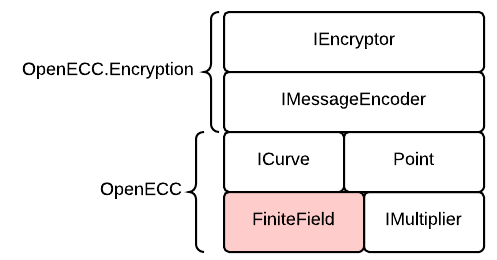
\includegraphics[width=0.7\textwidth]{implementation/components}
	\caption{The different components of the stack that enables encryption of a message.}
\end{figure}